\documentclass[10.5pt,a4paper]{article}
\usepackage[T1]{fontenc}
\usepackage[utf8]{inputenc}
\usepackage{mathpazo}
\usepackage[scaled=0.92]{helvet}
\usepackage[a4paper,margin=2.1cm]{geometry}
\usepackage{graphicx,booktabs,array,xcolor,enumitem,titlesec,caption,microtype,float}
\definecolor{accent}{HTML}{000000}
\titleformat{\section}{\Large\bfseries\sffamily\color{accent}}{\thesection}{0.6em}{}
\titleformat{\subsection}{\large\bfseries\sffamily}{\thesubsection}{0.6em}{}
\titlespacing*{\section}{0pt}{16pt}{8pt}
\titlespacing*{\subsection}{0pt}{11pt}{4pt}
\setlength{\parindent}{0pt}\setlength{\parskip}{6pt}
\setlist{itemsep=2pt,topsep=3pt,leftmargin=1.4em}
\captionsetup{font=small,labelfont=bf}
\renewcommand{\arraystretch}{1.15}

\begin{document}

{\sffamily\bfseries\huge\color{accent} Most Reliable Players Under Pressure\par}
\vspace{2pt}
{\sffamily\large How I ranked them, and who Rajasthan Royals should go after at the IPL 2027 auction\par}
\vspace{4pt}
{\small SupeRR Selector Season 2 \textperiodcentered{} Round 1 \textperiodcentered{} Romil\par}

\section{The short version}

Every cricket fan has an opinion on who is ``clutch''. I wanted to see what the ball-by-ball data says, and I wanted one number per player that answers a plain question: \emph{when the game is in the balance, how many runs is this player worth over an average one?}

My method has three parts. First I built a win-probability model and used it to find the balls that matter most to the result. The top quarter of those are my ``pressure balls''. Then I scored every ball against what an average player manages in the same situation. Finally, and this is the part I care about most, I checked my rating against matches it had never seen. A pressure ranking that does not repeat is only a list of who got lucky.

That check forced me to change course halfway through. My first rating used pressure balls only, and it fell apart when tested. The one in this report mixes a player's pressure record with his normal level, and it predicts unseen pressure performance about 50\% better. I describe what went wrong, and what I did about it, in Section~5.

\begin{table}[H]\centering\small
\begin{tabular}{c l l}
\toprule
Rank & Top 10 batters & Top 10 bowlers\\
\midrule
1 & Vaibhav Sooryavanshi & Kuldeep Yadav \\
2 & Abhishek Sharma & Rashid Khan \\
3 & Tim David & Sunil Narine \\
4 & Suryakumar Yadav & Jasprit Bumrah \\
5 & Heinrich Klaasen & Varun Chakravarthy \\
6 & Phil Salt & Mohammad Nawaz \\
7 & Andre Russell & Josh Hazlewood \\
8 & Cameron Green & Abrar Ahmed \\
9 & Jos Buttler & Mujeeb Ur Rahman \\
10 & Harry Brook & Mahedi Hasan\\
\bottomrule
\end{tabular}
\end{table}

For Rajasthan Royals the message is fairly blunt: the squad lacks bowlers who hold their nerve in tight overs, and it lacks a finisher in the middle order. Section~8 names the players I would bid for.

\section{The data}

I used only the data pack: roughly 201,000 deliveries from IPL 2022 to 2026 and T20 Internationals, along with the match, squad and competition files.

Some matches had to go. I removed no-results, abandoned games, ties and super overs, which left \textbf{769 matches and 181,002 deliveries}. For each ball I then rebuilt the state of the game as the bowler ran in: the score, wickets down, balls left, the target and the required rate. Rain-affected games needed care. I used the revised targets and overs from the match file, otherwise the required rates in those games would have been wrong.

\section{What I mean by pressure}

\subsection{Why not just use the death overs?}

That was my first instinct too, and it does not survive a few examples. Needing 12 an over is terrifying with three wickets left and fairly routine with nine in hand. The 19th over of a chase that is already gone has no pressure in it at all, even though it is a ``death over''. Required rate, wickets in hand, balls left: these are all hints at the same underlying thing, which is \emph{how much does this ball matter to who wins?} I decided to measure that directly.

\subsection{Step 1: a win-probability model}

I trained a gradient-boosted model to predict whether the batting side goes on to win. It sees the innings, runs, wickets down, balls remaining, runs needed, the current and required run rates, and a projected first-innings total. To keep it honest I used five-fold cross-validation grouped by match, so the probability for any ball comes from a model that never saw that match. On those held-out predictions the AUC is 0.80 and the Brier score is 0.18.

\subsection{Step 2: leverage}

For each ball I asked the model six what-ifs: what would the win probability be after a dot, a single, a two, a four, a six, or a wicket? I weighted them by how often each happens in T20 cricket (37\%, 36\%, 7\%, 11\%, 5\%, 4\%). If the six answers are far apart, the ball matters a lot. That spread is the ball's \textbf{leverage}. I scaled it so that an average ball scores 1.0, and I multiplied knockout matches by 1.2 because more is riding on them.

\subsection{Step 3: the cut-off}

A ball counts as high-pressure when its leverage is \textbf{1.35 or higher}. That is the top 25\% of all deliveries.

\subsection{Does it pick out the right balls?}

\begin{table}[H]\centering\small
\begin{tabular}{l c c}
\toprule
 & Normal balls & Pressure balls\\
\midrule
Deliveries & 135,751 & 45,251\\
Mean leverage & 0.67 & 2.09\\
Average win-probability swing per ball & 1.36\% & 4.39\%\\
Share that are in a chase & 41\% & 66\%\\
Runs per ball & 1.43 & 1.37\\
\bottomrule
\end{tabular}
\end{table}

A pressure ball shifts the match more than three times as far as a normal one, and batters score more slowly on them, which is what you would hope to see. One thing I did not expect: pressure is not mostly a death-overs story. In a chase, 44\% of powerplay balls are high-pressure, compared with 15\% in a first-innings powerplay. It makes sense once you think about it. Losing an opener early in a live chase hurts far more than conceding a boundary late in a game that is already settled.

\begin{figure}[H]\centering
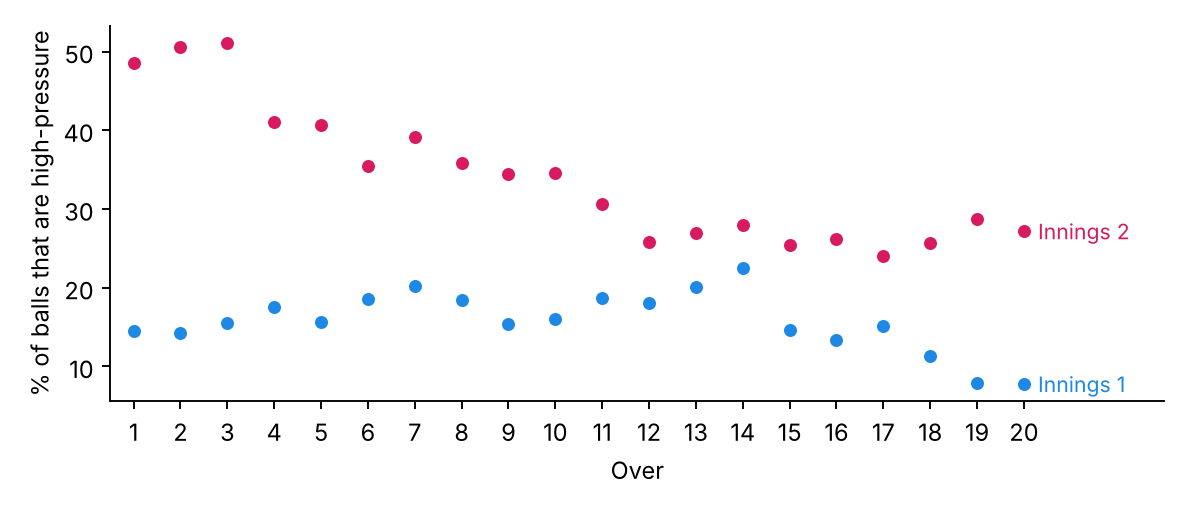
\includegraphics[width=0.78\textwidth]{c1_pressure_by_over.png}
\caption{Share of balls that are high-pressure, by over.}
\end{figure}

\section{Scoring a ball}

I compare every ball with the average for its situation. A situation here means the innings, the phase (powerplay, middle or death), how many wickets are down, whether it is a pressure ball, and whether the match is IPL or T20I.

\begin{itemize}
\item \textbf{For a batter:} runs scored minus the runs expected, with a penalty if he gets out (reduced by the chance that an average batter would have got out there anyway).
\item \textbf{For a bowler:} runs expected minus runs conceded, with a bonus for a wicket (reduced by the average chance of taking one).
\end{itemize}

That leaves the awkward question of how many runs a wicket is worth. I did not want to pick a number out of the air, so I read it off the win-probability model. Losing a wicket costs as much win probability as \textbf{6.1 runs on a pressure ball} and \textbf{8.9 runs on a normal ball}. Byes, leg-byes and run-outs are not held against the bowler. Wides and no-balls are.

Since the comparison always stays inside the same phase and the same kind of competition, an opener is never measured against a finisher, and an IPL innings is never measured against a T20I knock against a weak attack.

\section{The rating, and the test that shaped it}

\subsection{My first attempt, and why I dropped it}

The natural thing to do is rank players on their pressure balls and nothing else. That is what I built first, and the list looked believable enough.

Then I tried to break it. I split the matches into two random halves and rated every batter in each half separately. If the rating captured real skill, a batter who looked good in one half should look good in the other. He did not. The two sets of ratings had almost nothing to do with each other; the correlation was close to zero. A few hundred balls, a handful of which decide a match, is simply too little to separate skill from luck. The top 10 also reshuffled every time I moved the pressure cut-off slightly, which was a second warning.

\subsection{What I use instead}

For each player I calculate runs above average per 100 balls twice: once on his pressure balls and once on his normal balls. Both figures are pulled toward zero when the sample is small. In practice I add 300 average pressure balls and 200 average normal balls to every player before dividing. Then:

\begin{center}
\textbf{Pressure Reliability Rating = half the pressure level + half the normal level}
\end{center}

You can read it as \emph{the runs I expect this player to be worth, over an average player, per 100 pressure balls.} Both halves are shown for every player in the tables, so it is always clear how his pressure level compares with his usual one.

\subsection{Why half and half}

I did not choose the weights by feel. A hundred times over, I built ratings from a random half of the matches and compared them with what the same players actually did under pressure in the other half.

\begin{table}[H]\centering\small
\begin{tabular}{l c c}
\toprule
Rating built from & Batters & Bowlers\\
\midrule
Pressure balls only & 0.13 & 0.17\\
\textbf{Half pressure, half normal (used)} & \textbf{0.20} & \textbf{0.26}\\
\bottomrule
\end{tabular}
\caption*{\small Correlation with held-out pressure performance (Spearman).}
\end{table}

The blend is clearly better. If you want to know how someone will play under pressure, it helps a great deal to know how he plays the rest of the time. Any weight on pressure between a quarter and a half gives nearly the same accuracy. I went with a half because pressure balls are only a quarter of all balls, and I wanted them to count for more than their share.

\begin{figure}[H]\centering
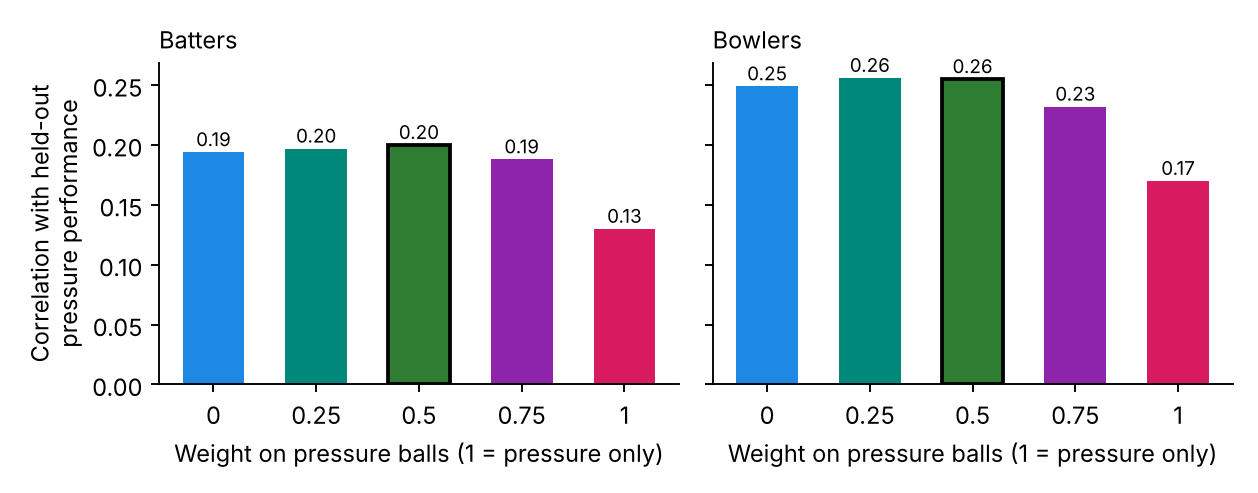
\includegraphics[width=0.8\textwidth]{c4_validation.png}
\caption{How well each weighting predicts pressure performance in unseen matches. The black outline marks the weighting I used.}
\end{figure}

\section{Keeping it fair}

\begin{itemize}
\item \textbf{Who qualifies:} a player needs at least 150 pressure balls, at least 15 matches with pressure involvement, and at least one match since January 2025. The last condition removes retired players. 86 batters and 92 bowlers make the cut.
\item \textbf{Small samples:} the added average balls drag thin records back toward the middle.
\item \textbf{IPL and T20Is:} both are included. Expected values are calculated separately for each, and a ball against an associate nation or an A side counts 0.6 as much as a ball against an IPL team or a full-member nation.
\item \textbf{Roles:} comparing within the same situation takes care of openers versus finishers and powerplay versus death bowlers.
\end{itemize}

\section{The top 10}

All values are runs better than average per 100 balls. ``+inns'' is the share of a player's pressure innings (or spells) in which he came out ahead. ``Top-10'' and ``Range'' come from resampling the matches, which I explain in Section~9.

\subsection{Batters}

\begin{figure}[H]\centering
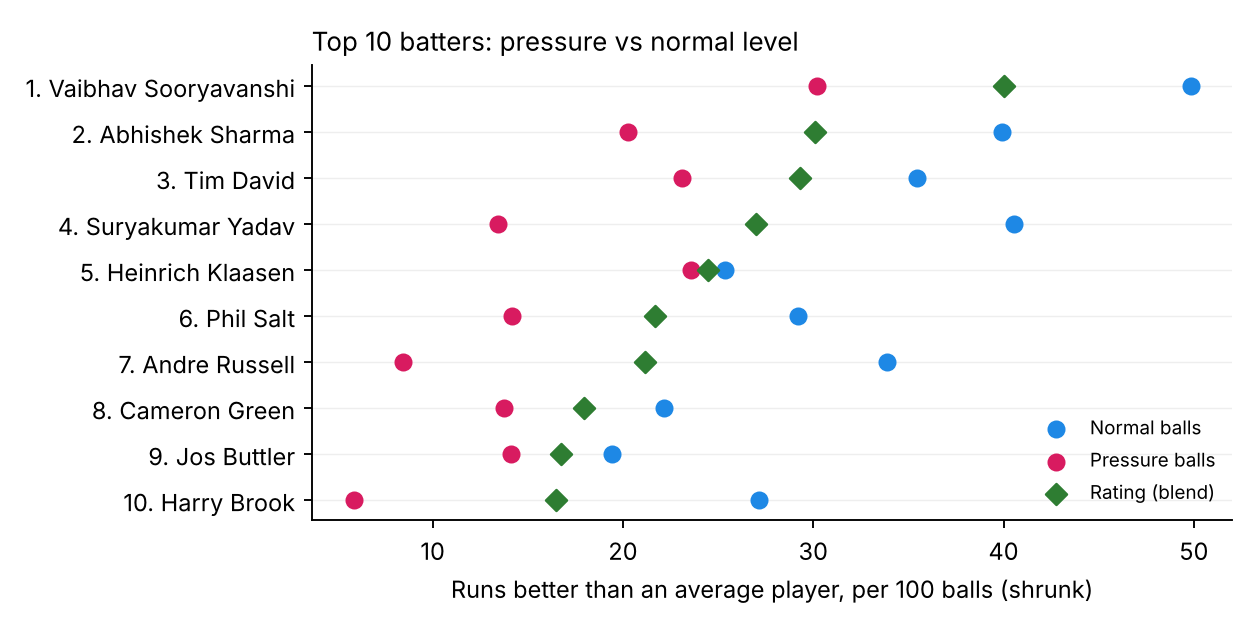
\includegraphics[width=0.86\textwidth]{c2_bat_top10.png}
\end{figure}

\begin{table}[H]\centering
\resizebox{\textwidth}{!}{%
\begin{tabular}{c l c c c c c c c c c c c c}
\toprule
\# & Batter & Rating & Pressure & Normal & Pr.\ balls & Pr.\ SR & Norm.\ SR & Pr.\ avg & Norm.\ avg & +inns & Top-10 & Range & IPL '26\\
\midrule
1 & Vaibhav Sooryavanshi & +40.0 & +30.2 & +49.8 & 174 & 232.8 & 221.0 & 45.0 & 43.0 & 65\% & 99\% & 1--4 & RR \\
2 & Abhishek Sharma & +30.1 & +20.3 & +39.9 & 531 & 179.7 & 191.5 & 29.8 & 36.9 & 58\% & 94\% & 1--9 & SRH \\
3 & Tim David & +29.3 & +23.1 & +35.5 & 359 & 168.5 & 181.6 & 37.8 & 33.8 & 59\% & 92\% & 1--10 & RCB \\
4 & Suryakumar Yadav & +27.0 & +13.4 & +40.6 & 577 & 151.0 & 176.0 & 34.8 & 44.4 & 50\% & 94\% & 2--9 & MI \\
5 & Heinrich Klaasen & +24.5 & +23.6 & +25.4 & 344 & 174.4 & 167.7 & 40.0 & 39.8 & 65\% & 87\% & 3--11 & SRH \\
6 & Phil Salt & +21.7 & +14.2 & +29.2 & 375 & 163.5 & 172.2 & 38.3 & 39.0 & 50\% & 70\% & 3--18 & RCB \\
7 & Andre Russell & +21.1 & +8.4 & +33.9 & 151 & 162.3 & 176.9 & 22.3 & 34.2 & 61\% & 60\% & 3--25 & -- \\
8 & Cameron Green & +18.0 & +13.8 & +22.2 & 258 & 163.6 & 153.6 & 35.2 & 47.7 & 50\% & 48\% & 5--26 & KKR \\
9 & Jos Buttler & +16.8 & +14.1 & +19.4 & 556 & 153.4 & 158.6 & 47.4 & 40.7 & 59\% & 30\% & 7--24 & GT \\
10 & Harry Brook & +16.5 & +5.8 & +27.2 & 205 & 151.7 & 169.1 & 25.9 & 42.5 & 52\% & 36\% & 5--40 & --\\
\bottomrule
\end{tabular}}
\end{table}

\begin{itemize}
\item \textbf{Sooryavanshi} is first, and it is not close. He strikes at 233 under pressure, averages more than he does in normal play, and stays in the top 10 in 99\% of resamples. He has only 174 pressure balls, so I was ready for the shrinkage to knock him down. It did not.
\item \textbf{Klaasen} is the batter whose game barely changes: +23.6 under pressure against +25.4 normally, and his strike rate actually rises.
\item \textbf{Tim David} is the best finisher in the data. He strikes at 200 across 141 pressure balls at the death.
\item \textbf{Suryakumar and Brook} are in the list on class. Both dip under pressure, though they stay above average.
\end{itemize}

\subsection{Bowlers}

\begin{figure}[H]\centering
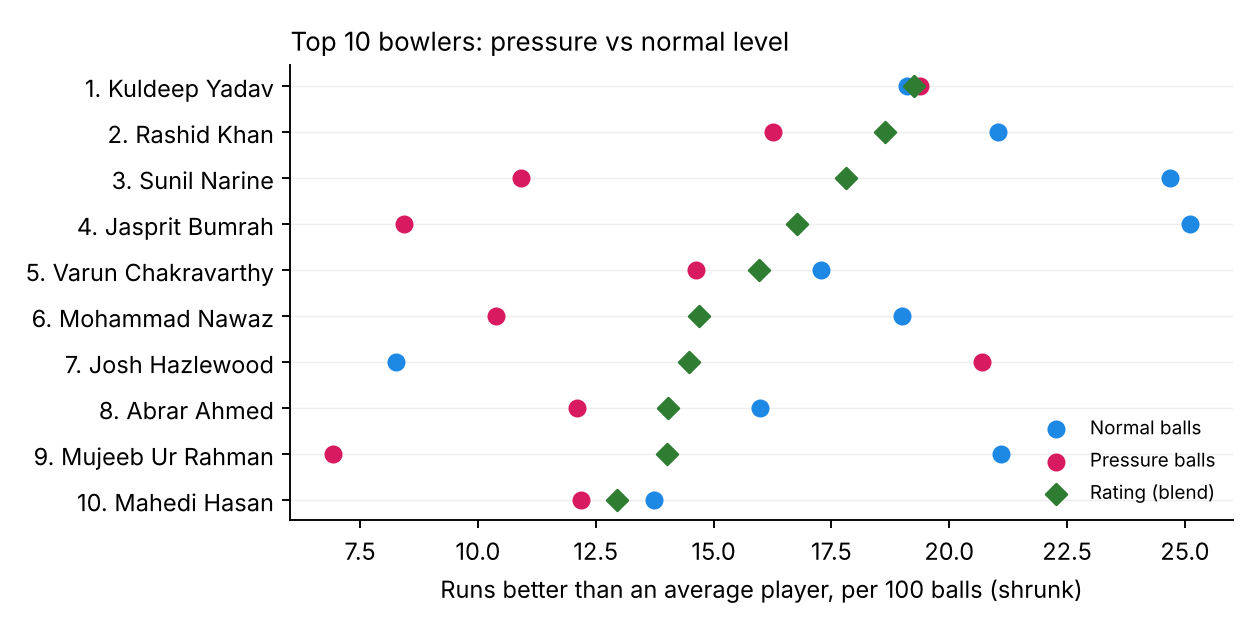
\includegraphics[width=0.86\textwidth]{c3_bowl_top10.png}
\end{figure}

\begin{table}[H]\centering
\resizebox{\textwidth}{!}{%
\begin{tabular}{c l c c c c c c c c c c c c}
\toprule
\# & Bowler & Rating & Pressure & Normal & Pr.\ balls & Wkts & Pr.\ econ & Norm.\ econ & Dot \% & +spells & Top-10 & Range & IPL '26\\
\midrule
1 & Kuldeep Yadav & +19.2 & +19.4 & +19.1 & 430 & 33 & 7.33 & 7.91 & 35.3 & 61\% & 82\% & 1--14 & DC \\
2 & Rashid Khan & +18.6 & +16.3 & +21.0 & 564 & 34 & 7.17 & 7.25 & 34.4 & 64\% & 82\% & 1--15 & GT \\
3 & Sunil Narine & +17.8 & +10.9 & +24.7 & 316 & 12 & 6.93 & 6.83 & 38.6 & 69\% & 79\% & 2--15 & KKR \\
4 & Jasprit Bumrah & +16.8 & +8.4 & +25.1 & 398 & 15 & 7.30 & 7.34 & 44.7 & 63\% & 67\% & 1--19 & MI \\
5 & Varun Chakravarthy & +16.0 & +14.6 & +17.3 & 456 & 29 & 7.29 & 8.17 & 40.1 & 65\% & 64\% & 2--19 & KKR \\
6 & Mohammad Nawaz & +14.7 & +10.4 & +19.0 & 304 & 25 & 7.70 & 6.87 & 35.9 & 55\% & 56\% & 2--28 & -- \\
7 & Josh Hazlewood & +14.5 & +20.7 & +8.3 & 440 & 33 & 7.46 & 8.49 & 47.7 & 63\% & 56\% & 2--31 & RCB \\
8 & Abrar Ahmed & +14.0 & +12.1 & +16.0 & 234 & 15 & 6.49 & 6.77 & 39.3 & 65\% & 49\% & 2--31 & -- \\
9 & Mujeeb Ur Rahman & +14.0 & +6.9 & +21.1 & 251 & 13 & 7.27 & 6.93 & 39.8 & 58\% & 51\% & 3--28 & -- \\
10 & Mahedi Hasan & +13.0 & +12.2 & +13.7 & 227 & 14 & 6.53 & 7.22 & 44.5 & 67\% & 44\% & 3--31 & --\\
\bottomrule
\end{tabular}}
\end{table}

\begin{itemize}
\item \textbf{Kuldeep} is the same bowler whatever the situation (+19.4 and +19.1), and he takes a wicket every 13 pressure balls.
\item \textbf{Hazlewood} is the one who lifts. He is +20.7 under pressure against +8.3 normally, and his economy drops by a full run.
\item \textbf{Narine, Bumrah and Mujeeb} are outstanding in normal play and good, rather than great, under pressure. The rating gives them credit for both.
\item Eight of the ten are spinners. I do not think that is a quirk. Most pressure balls come in chases and through the middle overs, and that is where a good spinner takes hold of a game.
\end{itemize}

\section{What this means for Rajasthan Royals}

\subsection{The auction}

The IPL 2027 auction is a one-day mini-auction in Goa on 16 December 2026, and franchises have until 17 November to hand in their retained and released lists (as reported by ESPNcricinfo). I wrote this before the pool was known. So I have taken availability from the data pack itself: ``--'' means the player was not in any IPL 2026 squad, and a team code means he was contracted there and can only be bought if he is released or traded.

\subsection{Where the squad is short}

Below is every Royals player who qualifies, ranked against all 86 eligible batters and 92 eligible bowlers.

\begin{table}[H]\centering\small
\begin{tabular}{l c c c c}
\toprule
RR batter & Rank & Pressure & Normal & Pr.\ SR\\
\midrule
Vaibhav Sooryavanshi & 1 & +30.2 & +49.8 & 232.8 \\
Yashasvi Jaiswal & 20 & +12.9 & +11.2 & 169.5 \\
Ravindra Jadeja & 39 & +8.7 & +2.8 & 136.7 \\
Shimron Hetmyer & 40 & +6.4 & +4.9 & 148.7 \\
Dasun Shanaka & 42 & +10.7 & +0.0 & 150.0 \\
Dhruv Jurel & 49 & $-$3.0 & +11.5 & 138.8 \\
Riyan Parag & 54 & $-$3.1 & +8.7 & 143.8 \\
Sam Curran & 79 & +3.6 & $-$12.2 & 131.2\\
\bottomrule
\end{tabular}

\vspace{8pt}
\begin{tabular}{l c c c c c}
\toprule
RR bowler & Rank & Pressure & Normal & Pr.\ econ & Death pr.\ econ (balls)\\
\midrule
Ravi Bishnoi & 45 & $-$4.5 & +5.5 & 8.39 & 9.9 (63) \\
Jofra Archer & 51 & $-$4.5 & +3.4 & 9.40 & 9.4 (61) \\
Ravindra Jadeja & 57 & +6.9 & $-$8.9 & 7.18 & 17.0 (6) \\
Sandeep Sharma & 67 & $-$7.0 & +0.8 & 9.01 & 12.4 (66) \\
Sam Curran & 89 & $-$14.8 & $-$12.7 & 9.89 & 9.5 (104)\\
\bottomrule
\end{tabular}
\end{table}

Two things jump out.

\textbf{Bowling under pressure is the weak spot.} Not one Royals bowler is in the top 40, and four of the five are below average on pressure balls. Season reviews of RR's 2026 campaign said much the same from the outside: there was no second strike bowler to share the load with Archer.

\textbf{The top order is settled; the middle is not.} Sooryavanshi is first and Jaiswal is 20th. Hetmyer, Jurel and Parag are all somewhere between 40th and 54th.

\subsection{Need 1: a bowler for the tight overs}

\begin{table}[H]\centering
\resizebox{\textwidth}{!}{%
\begin{tabular}{l l c c c c c c}
\toprule
Target & Style & Rank & Pressure & Econ pr.\ / normal & Death pr.\ econ (balls) & IPL pr.\ balls & IPL '26\\
\midrule
\multicolumn{8}{l}{\emph{Pace}}\\
Taskin Ahmed & RA Fast & 18 & +7.9 & 6.98 / 8.29 & 7.5 (63) & 0 & -- \\
FazalHaq Farooqi & LA medium & 46 & +11.1 & 7.27 / 8.57 & 8.2 (54) & 19 & -- \\
Josh Hazlewood & RA fast-medium & 7 & +20.7 & 7.46 / 8.49 & 9.2 (72) & 283 & RCB \\
Trent Boult & LA fast-medium & 19 & +15.9 & 7.51 / 8.83 & 7.8 (54) & 348 & MI \\
Nathan Ellis & RA medium & 15 & +8.2 & 8.09 / 8.11 & 10.8 (73) & 97 & CSK \\
Blessing Muzarabani & RA fast-medium & 13 & +8.2 & 7.39 / 7.56 & 11.3 (41) & 14 & KKR\\
\midrule
\multicolumn{8}{l}{\emph{Spin}}\\
Mujeeb Ur Rahman & RA offbreak & 9 & +6.9 & 7.27 / 6.93 & 7.6 (23) & 0 & -- \\
Mahedi Hasan & RA offbreak & 10 & +12.2 & 6.53 / 7.22 & 10.9 (16) & 0 & -- \\
Adil Rashid & RA Leg-Break & 30 & +10.9 & 6.83 / 8.17 & 8.4 (30) & 6 & --\\
\bottomrule
\end{tabular}}
\end{table}

\begin{itemize}
\item \textbf{Taskin Ahmed} would be my first call among players outside the IPL 2026 squads. He bowls fast, goes at 7.0 an over under pressure against 8.3 normally, and concedes 7.5 in death-over pressure. That is precisely where Archer and Sandeep Sharma have been expensive. The catch is that everything I have on him is from T20Is.
\item \textbf{Hazlewood and Boult}, if either comes into the pool, are the two fast bowlers in this data who clearly improve under pressure. Either would be the second strike bowler RR has been missing, and Boult already knows the dressing room.
\item \textbf{Farooqi} is a cheaper left-arm option (+11.1 under pressure).
\item \textbf{Mujeeb} bowls 61\% of his pressure balls in the powerplay. Having him take those overs would let RR save Archer for the end.
\end{itemize}

\subsection{Need 2: a middle-order finisher}

\begin{table}[H]\centering
\resizebox{\textwidth}{!}{%
\begin{tabular}{l c c c c c c c c c}
\toprule
Target & Hand & Rank & Pressure & Pr.\ SR & Pr.\ avg & Death pr.\ SR (balls) & Chase pr.\ avg & IPL pr.\ balls & IPL '26\\
\midrule
Harry Brook & RHB & 10 & +5.8 & 151.7 & 25.9 & 231 (26) & 20.2 & 24 & -- \\
Daryl Mitchell & RHB & 30 & +10.9 & 139.5 & 51.2 & 156 (16) & 76.5 & 25 & -- \\
Tim David & RHB & 3 & +23.1 & 168.5 & 37.8 & 200 (141) & 30.8 & 140 & RCB \\
Heinrich Klaasen & RHB & 5 & +23.6 & 174.4 & 40.0 & 230 (56) & 32.6 & 284 & SRH \\
David Miller & LHB & 14 & +13.6 & 151.4 & 45.4 & 190 (110) & 46.6 & 263 & DC \\
Rovman Powell & RHB & 18 & +11.4 & 157.0 & 26.6 & 197 (118) & 29.7 & 101 & KKR\\
\bottomrule
\end{tabular}}
\end{table}

\begin{itemize}
\item \textbf{Daryl Mitchell} is the man for a chase. He averages 76 in pressure chases, and he is one of the few players whose pressure level (+10.9) is higher than his normal one.
\item \textbf{Harry Brook} is 10th overall on class and was not in an IPL 2026 squad. I would be careful, though. Under pressure he is only slightly above average, and nearly all of his record here is from T20Is. Buying him is a bet on talent.
\item \textbf{David, Klaasen, Miller and Powell} are all under contract elsewhere. If David (death strike rate 200) or Klaasen (no drop under pressure) is released, I would spend big.
\end{itemize}

\subsection{Three cautions}

\begin{itemize}
\item \textbf{Andre Russell} and the \textbf{Pakistan players} in my bowling list (Nawaz and Abrar) have earned their ranks on the numbers, but they are not realistic IPL 2027 signings. Russell was not in an IPL 2026 squad, and Pakistan players have not appeared in the IPL since 2008.
\item Players with \textbf{no IPL pressure balls} in this data (Taskin, Mujeeb, Mahedi) should be priced with that uncertainty in mind.
\item The shortlist should be run again once the official pool is out. My ranked tables list every eligible player with his 2026 team, so that is a quick job.
\end{itemize}

\section{How far to trust this}

\begin{figure}[H]\centering
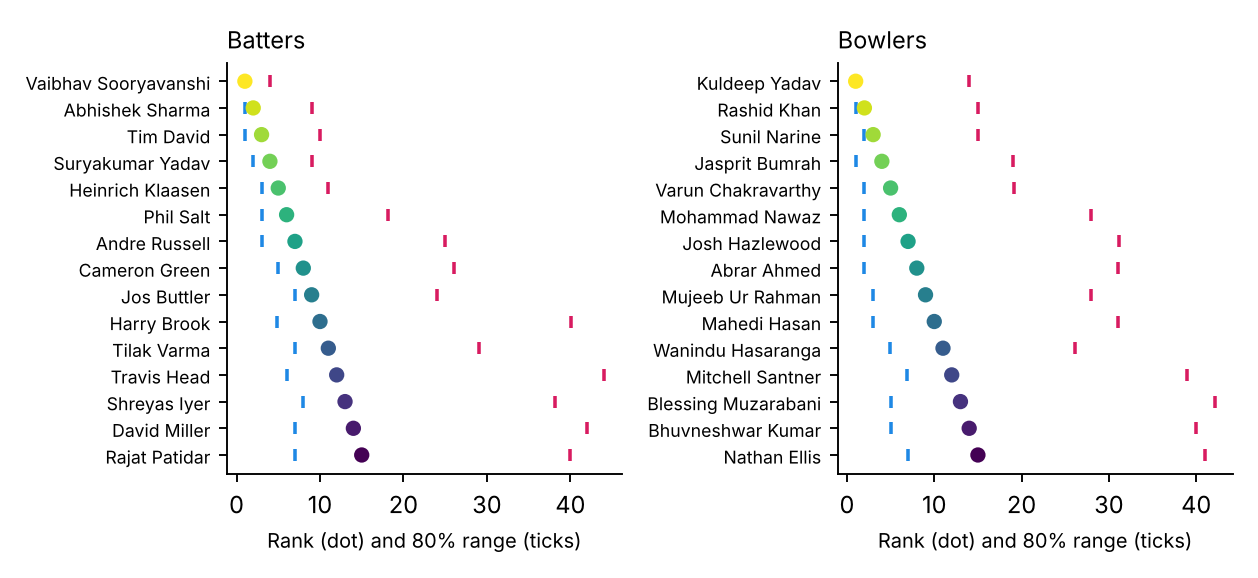
\includegraphics[width=0.86\textwidth]{c5_rank_uncertainty.png}
\caption{Each player's rank (dot), with a blue tick and a pink tick marking the two ends of the range it fell in across 80\% of resamples.}
\end{figure}

I would rather be upfront about how solid these rankings are.

\begin{itemize}
\item \textbf{Prediction on unseen matches:} 0.20 for batters and 0.26 for bowlers. Those are not big numbers. Pressure performance is noisy whichever way you measure it. What matters is that this rating does about 50\% better than the pressure-only version.
\item \textbf{Resampling:} I redrew the 769 matches 400 times and ranked everyone again each time. The top five in each list land in the top 10 at least 64\% of the time. Ranks 8 to 10 are closer to 30--50\%, so they are not far ahead of the players just below them.
\item \textbf{Moving the cut-off:} if I use the top 30\% or the top 20\% of balls instead of 25\%, 9 and 10 of my top 10 batters stay, and 9 and 10 of my top 10 bowlers stay.
\item \textbf{Consistency from match to match:} every player in both top 10s comes out ahead in at least half of his pressure innings or spells.
\item \textbf{Looking forward in time:} I rated players using only matches before 2025 and compared that with how they did under pressure in 2025--26. For bowlers the link is positive (+0.17, from 50 players). For batters it is $-$0.14 (49 players), which is no better than chance. Batting form did not carry across that gap, so I have more faith in my bowling list than in my batting list.
\end{itemize}

\section{Limits}

\begin{itemize}
\item Even the better rating explains only a small part of future pressure performance. The ranking is an informed ordering and should be read that way.
\item The pressure figure is shrunk harder than the normal one because there are fewer pressure balls. As a result each player's pressure-versus-normal gap probably looks a bit worse than it is.
\item The win-probability model knows nothing about the venue, the pitch, the quality of the two teams or who is at the crease.
\item Only the striker and the bowler get credit. Fielding and partnerships are left out.
\item The 25\% cut-off, the 0.6 opposition weight and the shrinkage sizes are my own judgement calls. I tested the blend weight. I did not tune the others.
\item The data pack has nothing on age, fitness, price or who will actually be in the auction.
\end{itemize}

\section{Reproducing the work}

All the numbers in this report come from one Python script, which cleans the data, fits the win-probability model, computes leverage and the ratings, and runs the validation checks. It takes about two minutes and uses fixed random seeds, so it gives the same answer every time. A second short script draws the figures. I can share the code and the full ranked tables for every eligible player on request.

\textbf{Public information used in Section 8:} ESPNcricinfo's report on the IPL 2027 retention deadline (auction date, format and deadlines), and published season reviews of RR's IPL 2026 campaign.

\end{document}
